\documentclass[8pt]{beamer}
\usepackage{tikz}
\usepackage[utf8]{vietnam}
\usepackage{amsmath}
\usepackage{graphicx}
\usepackage{wrapfig}
\usepackage{hyperref}
\usepackage{mathrsfs}
\usetheme{Copenhagen}
\usecolortheme{dolphin}
\setbeamertemplate{navigation symbols}{}
\setbeamertemplate{headline}{}
\title[Chương 3: Biến đổi Fourier nhanh (FFT)] %optional
{Chương 3: Biến đổi Fourier nhanh (FFT)}
\subtitle{Xử lý tín hiệu số}
\author[Xử lý tín hiệu số] % (optional)
{Tín Vũ}
\date[VLC 2021] % (optional)
{tinvu1309@gmail.com}
\begin{document}
\frame{\titlepage}
\begin{frame}{Mục lục}
\tableofcontents
\end{frame}
\begin{frame}{Giới thiệu playlist}
\section{Giới thiệu playlist}
	\begin{itemize}
		\item Mình là Tín Vũ, hiện đang là sinh viên học tại Trường Đại học Công nghệ, Đại học Quốc gia Hà Nội. Mình tạo playlist video này để hỗ trợ các bạn học môn \textbf{Xử lý tín hiệu số}.
\item Khác với môn học tiên quyết \alert{Tín hiệu hệ thống} trước đó, bài giảng môn học này \textbf{hoàn toàn bám sát với đề cương và giáo trình nội bộ} của trường mình, nên các bạn trường khác cần phải lưu ý rất kĩ điều này.
\item Không chỉ dừng lại ở lý thuyết, playlist này \textbf{có bổ sung hướng dẫn lập trình cơ bản bằng GNU Octave/Matlab} để vẽ phổ tín hiệu, đáp ứng tần số và thiết kế bộ lọc.
\item Môn học này bao gồm \textbf{6 chương}, các chương đều liên quan rất chặt chẽ với nhau nên hãy học cẩn thận ngay từ \alert{Chương 0} để ôn thi cuối kì đỡ vất vả.
	\end{itemize}
\end{frame}
\begin{frame}{Tài liệu tham khảo}
\section{Tài liệu tham khảo}
\begin{itemize}
		\item Tài liệu tham khảo chính: Giáo trình Xử lý tín hiệu số (Nguyễn Linh Trung, Trần Đức Tân, Huỳnh Hữu Tuệ, ĐHCN, 2012).
		\item Tài liệu tham khảo phụ: Discrete-time Signal Processing (Alan V.Oppenheim, 2nd edition). 
	\end{itemize}
\end{frame}
\begin{frame}{Quy trình xử lý tín hiệu số}
\section{Quy trình xử lý tín hiệu số}
\begin{figure}[h]
			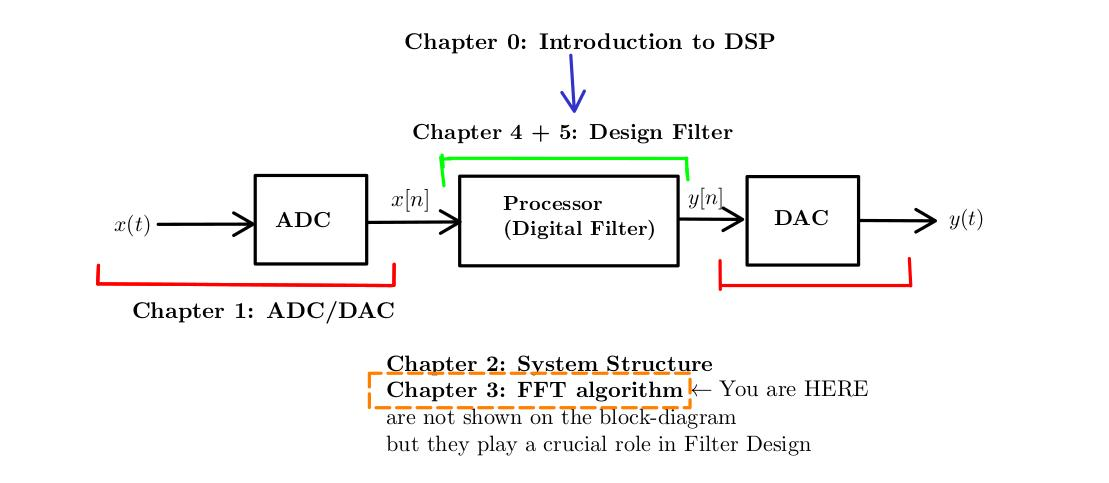
\includegraphics[width=1.1\textwidth]{1.jpg}
			\caption{DSP Learning Process}			\label{fig:re1}
		\end{figure}

\end{frame}
\begin{frame}{Biến đổi Fourier rời rạc (DFT)}
\section{Biến đổi Fourier rời rạc (DFT)}
Trong học phần \alert{Tín hiệu hệ thống} trước đó, ta đã biết $2$ cặp công thức gồm chuỗi Fourier thời gian rời rạc (DTFS) và biến đổi Fourier thời gian rời rạc (DTFT):
\begin{enumerate}
	\item[1]  DTFS pairs: $$x[n]=\sum_{k=<N_{0}>}c_{k}e^{jk\omega_{0}n}$$
		$$c_{k}=\frac{1}{N_{0}}\sum_{n=<N_{0}>}x[n]e^{-jk\omega_{0}n}$$
	\item[2] DTFT pairs: $$x[n]=\frac{1}{2\pi}\int_{2\pi}X(\omega)e^{j\omega n}d\omega$$
		$$X(\omega)=\sum_{n=-\infty}^{+\infty}x[n]e^{-j\omega n}$$
\end{enumerate}
Ta thấy DTFS chỉ có thể được sử dụng để phân tích \textbf{tín hiệu rời rạc tuần hoàn}, còn DTFT chỉ được dùng khi phân tích \textbf{tín hiệu rời rạc không tuần hoàn vô hạn}. Không chỉ có vậy, để phân tích bằng DTFS hay DTFT, tín hiệu đầu vào \textbf{phải là một hàm số theo biến thời gian $n$}.
\\ Hiển nhiên ta thấy rằng trong thực tiễn, \alert{không có dạng tín hiệu hoàn hảo nào thỏa mãn đủ điều kiện để phân tích DTFS hay DTFT}. Các tín hiệu trong thực tiễn thường ở dạng \alert{ngẫu nhiên} (không thể mô hình hóa bằng một hàm số), \alert{không tuần hoàn}, \alert{độ dài hữu hạn} (có khi độ dài cực kì ngắn).
\\ Trong chương này, ta sẽ phát triển công thức và thuật toán để xác định phổ của tín hiệu trong thực tế.
\end{frame}
\begin{frame}{Biến đổi Fourier rời rạc (DFT)}
Dựa vào công thức DTFS và DTFT, các nhà toán học đã phát triển cặp công thức DFT (discrete Fourier transform pair) như sau:
$$x[n]=\frac{1}{N_{0}}\sum_{\alert{k=0}}^{\alert{N_{0}-1}}X[k]e^{jk\omega_{0}n}=\frac{1}{N_{0}}\sum_{\alert{k=0}}^{\alert{N_{0}-1}}X[k]e^{jk\frac{2\pi}{N_{0}}n}$$
$$X[k]=\sum_{\alert{n=0}}^{\alert{N_{0}-1}}x[n]e^{-jk\omega_{0}n}=\sum_{\alert{n=0}}^{\alert{N_{0}-1}}x[n]e^{-jk\frac{2\pi}{N_{0}}n}$$
Chúng ta phải phân biệt rất rạch ròi bản chất toán học của các công thức DTFS, DTFT và DFT, tuyệt đối không được nhầm lẫn chúng với nhau. 
\\ Nếu ta kí hiệu: $$W_{N_{0}}=e^{-j\frac{2\pi}{N_{0}}}$$
Ta có thể viết lại các công thức DFT như sau:
$$x[n]=\frac{1}{N_{0}}\sum_{k=0}^{N_{0}-1}X[k]W_{N_{0}}^{-kn}$$
$$X[k]=\sum_{n=0}^{N_{0}-1}x[n]W_{N_{0}}^{kn}$$
\end{frame}
\begin{frame}{Biến đổi Fourier rời rạc (DFT)}
Để cho dễ nhìn hơn, ta viết lại công thức DFT dưới dạng tích ma trận:
\begin{equation*}
	\begin{bmatrix}
		X[0]\\
		X[1]\\
		X[2]\\
		\cdots\\
		X[N_{0}-2]\\
		X[N_{0}-1]\\
	\end{bmatrix}
	=
	\begin{bmatrix}
		1&&1&&1&&\cdots&&1\\
		1&&W_{N_{0}}^{1}&&W_{N_{0}}^{2}&&\cdots&&W_{N_{0}}^{N_{0}-1}\\
		1&&W_{N_{0}}^{2}&&W_{N_{0}}^{4}&&\cdots&&W_{N_{0}}^{2(N_{0}-1)}\\
		\cdots&&\cdots&&\cdots&&\cdots&&\cdots\\
		1&&W_{N_{0}}^{N_{0}-2}&&W_{N_{0}}^{2(N_{0}-2)}&&\cdots&& W_{N_{0}}^{(N_{0}-2)(N_{0}-1)}\\
		1&&W_{N_{0}}^{N_{0}-1}&&W_{N_{0}}^{2(N_{0}-1)}&&\cdots&&W_{N_{0}}^{(N_{0}-1)^2}\\
	\end{bmatrix}
	\begin{bmatrix}
		x[0]\\x[1]\\x[2]\\ \cdots\\x[n-2]\\x[n-1]
	\end{bmatrix}
\end{equation*}
Hiển nhiên ta thấy $W_{N_{0}}^{-kn}=W_{N_{0}}^{kn^{*}}$, vậy ta viết lại công thức IDFT dưới dạng tích ma trận:
\begin{equation*}
	\begin{bmatrix}
		x[0]\\
		x[1]\\
		x[2]\\
		\cdots\\
		x[N_{0}-2]\\
		x[N_{0}-1]\\
	\end{bmatrix}
	=\alert{\frac{1}{N_{0}}}
	\begin{bmatrix}
		1&&1&&\cdots&&1\\
		1&&W_{N_{0}}^{1^*}&&\cdots&&W_{N_{0}}^{(N_{0}-1)^*}\\
		1&&W_{N_{0}}^{2^*}&&\cdots&&W_{N_{0}}^{2(N_{0}-1)^*}\\
		\cdots&&\cdots&&\cdots&&\cdots\\
		1&&W_{N_{0}}^{(N_{0}-2)^*}&&\cdots&& W_{N_{0}}^{(N_{0}-2)(N_{0}-1)^*}\\
		1&&W_{N_{0}}^{(N_{0}-1)^*}&&\cdots&&W_{N_{0}}^{(N_{0}-1)^2^{*}}\\
	\end{bmatrix}
	\begin{bmatrix}
		X[0]\\X[1]\\X[2]\\ \cdots\\X[n-2]\\X[n-1]
	\end{bmatrix}
\end{equation*}
\end{frame}
\begin{frame}{Biến đổi Fourier rời rạc (DFT)}
\begin{figure}[h]
			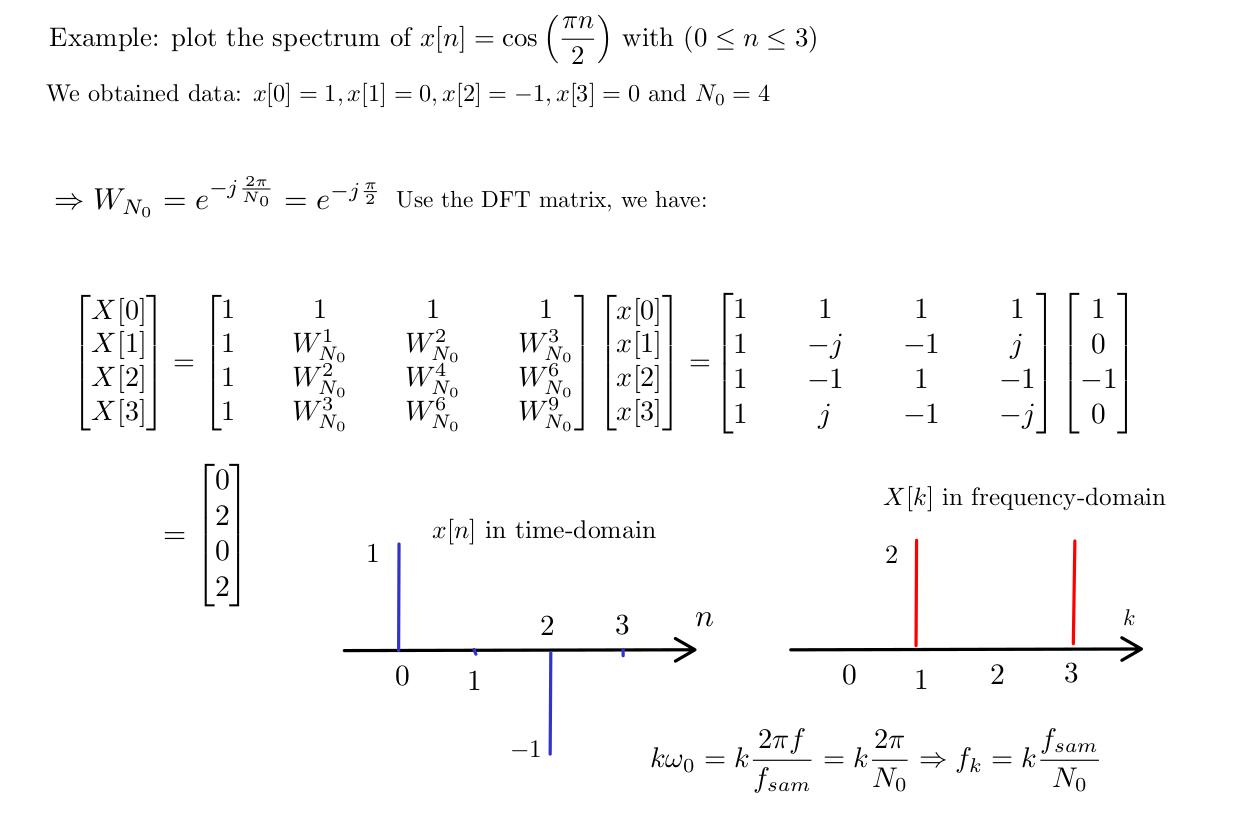
\includegraphics[width=1\textwidth]{2.jpg}

			\caption{DFT matrix}			\label{fig:re2}

		\end{figure}


\end{frame}
\begin{frame}{Biến đổi Fourier rời rạc (DFT)}
\begin{figure}[h]
			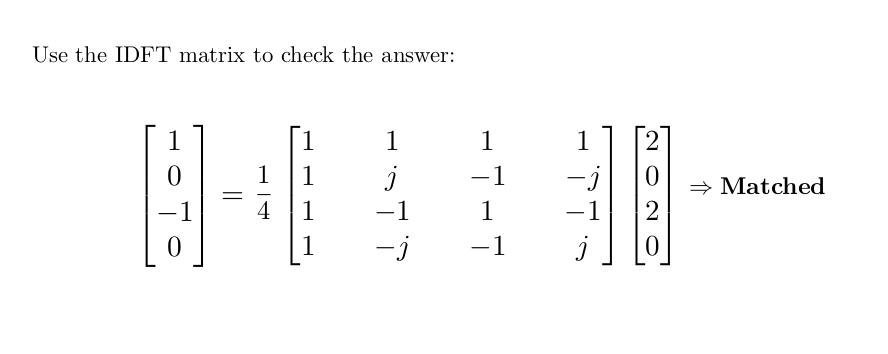
\includegraphics[width=0.7\textwidth]{3.jpg}

			\caption{IDFT matrix}			\label{fig:re3}

		\end{figure}

Đương nhiên, các bạn hoàn toàn có thể chọn các tín hiệu rời rạc với dữ liệu khác để thay vào công thức DFT và IDFT để kiếm tra kết quả tính toán; ở đây mình chỉ chọn ví dụ đơn giản nhất để minh họa. 
\\ Trong quá trình DFT của tín hiệu trong ví dụ trên, chúng ta đã phải thực hiện $4.4=16$ phép nhân và $3.4=12$ phép cộng, tổng là $17+12=28$ phép toán cho ma trận $4x4$ (hay DFT 4 điểm). Kết quả này hoàn toàn tương tự với IDFT.
\\ Tổng quát, nếu ma trận $NxN$ (hay DFT/IDFT) $N$ điểm, ta sẽ phải thực hiện $N^2$ phép nhân và $N(N-1)$ phép cộng, ta dễ thấy độ phức tạp của thuật toán này là $\mathscr{O}(N^2)$.
\\ Năm 1965, hai nhà toán học người Mỹ J.W.Cooley và John Tukey đã phát triển thuật toán biến đổi Fourier nhanh (fast Fourier transform) giảm độ phức tạp của thuật toán còn $\mathscr{O}{(N\log_{2}N)}$.
\end{frame}
\begin{frame}{Biến đổi Fourier nhanh (FFT)}
	\section{Biến đổi Fourier nhanh (FFT)}
	Thuật toán biến đổi Fourier nhanh (từ giờ ta sẽ gọi tắt là FFT) rất phức tạp để có thể giải thích toàn bộ (và cũng vượt quá yêu cầu môn học), nên ta chỉ nghiên cứu thuật toán FFT đơn giản nhất là \textbf{phân rã trong miền thời gian} (decimation in time - DIT, radix 2), vẽ lưu đồ dòng chảy cho tín hiệu $4$, $8$ và phát triển giải thuật cho $N$ điểm. Cuối cùng, chương này kết thúc với sử dụng phần mềm mô phỏng (GNU Octave/Matlab) thực thi thuật toán FFT.
\\ Ta xét công thức DFT: $$X[k]=\sum_{n=0}^{N_{0}-1}x[n]W_{N_{0}}^{kn}$$
Ta liên tục tách nhỏ $X[k]$ nhằm tạo các "cặp" phân rã theo cơ số 2 như sau:
\end{frame}
\begin{frame}{Biến đổi Fourier nhanh (FFT)}
\begin{equation*}
\begin{split}
	X[k]&=\sum_{n=0}^{N_{0}-1}x[n]W_{N_{0}}^{kn}=\sum_{r=0}^{\frac{N_{0}}{2}-1}x[2r]W_{N_{0}}^{k2r}+\sum_{r=0}^{\frac{N_{0}}{2}-1}x[2r+1]W_{N_{0}}^{k(2r+1)}\\
	    &=\sum_{r=0}^{\frac{N_{0}}{2}-1}x[2r]W_{\frac{N_{0}}{2}}^{kr}+W_{N_{0}}^{k}\sum_{r=0}^{\frac{N_{0}}{2}-1}x[2r+1]W_{\frac{N_{0}}{2}}^{kr}=\alert{X_{\text{n even}}[k]+W_{N_{0}}^{k}X_{\text{n odd}}[k]}\\
	    &=\left(\sum_{r=0}^{\frac{N_{0}}{4}-1}x[4r]W_{\frac{N_{0}}{2}}^{k2r}+\sum_{r=0}^{\frac{N_{0}}{4}-1}x[4r+2]W_{\frac{N_{0}}{2}}^{k(2r+1)}\right)+\\ &W_{N_{0}}^{k}\left(\sum_{r=0}^{\frac{N_{0}}{4}-1}x[4r+1]W_{\frac{N_{0}}{2}}^{k2r} +\sum_{r=0}^{\frac{N_{0}}{4}-1}x[4r+3]W_{\frac{N_{0}}{2}}^{k(2r+1)} \right)\\
	    &=\left(\sum_{r=0}^{\frac{N_{0}}{4}-1}x[4r]W_{\frac{N_{0}}{4}}^{kr}+W_{\frac{N_{0}}{2}}^{k}\sum_{r=0}^{\frac{N_{0}}{4}-1}x[4r+2]W_{\frac{N_{0}}{4}}^{kr}\right)+\\ &W_{N_{0}}^{k}\left(\sum_{r=0}^{\frac{N_{0}}{4}-1}x[4r+1]W_{\frac{N_{0}}{4}}^{kr}+W_{\frac{N_{0}}{2}}^{k}\sum_{r=0}^{\frac{N_{0}}{4}-1}x[4r+3]W_{\frac{N_{0}}{4}}^{kr}\right)
\end{split}
\end{equation*}
\end{frame}
\begin{frame}{Biến đổi Fourier nhanh (FFT)}
Ta thấy do tính tuần hoàn:
$$X_{\text{n even}}[k]=X_{\text{n even}}\left[k+\frac{N_{0}}{2}\right]$$

$$X_{\text{n odd}}[k]=X_{\text{n odd}}\left[k+\frac{N_{0}}{2}\right]$$
Vậy từ tất cả các biến đổi cơ bản trên, ta có thể vẽ lại thành một sơ đồ phân rã hình cây nhị phân 3 tầng như sau:
\end{frame}
\begin{frame}{Biến đổi Fourier nhanh (FFT)}
\begin{figure}[h]
			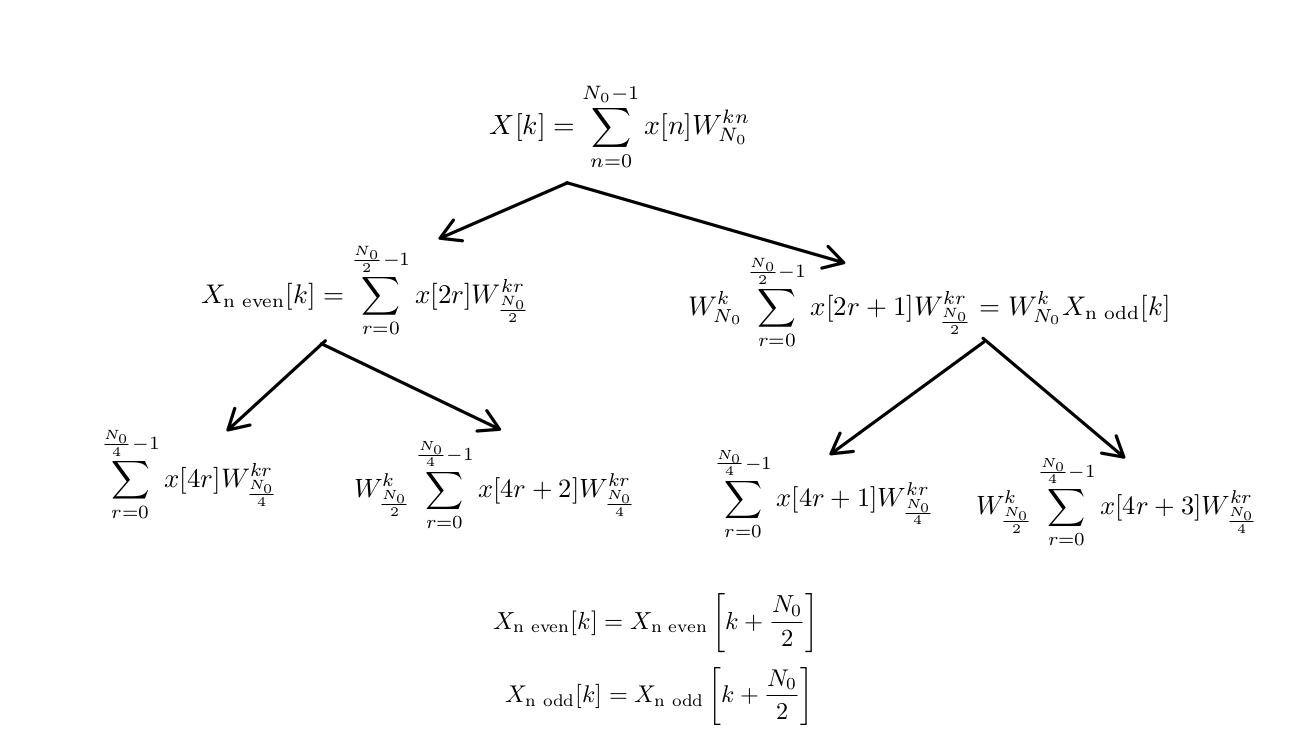
\includegraphics[width=1.1\textwidth]{4.jpg}

			\caption{DFT radix 2 binary tree}			\label{fig:re4}

		\end{figure}


\end{frame}
\begin{frame}{Biến đổi Fourier nhanh (FFT)}
\begin{figure}[h]
			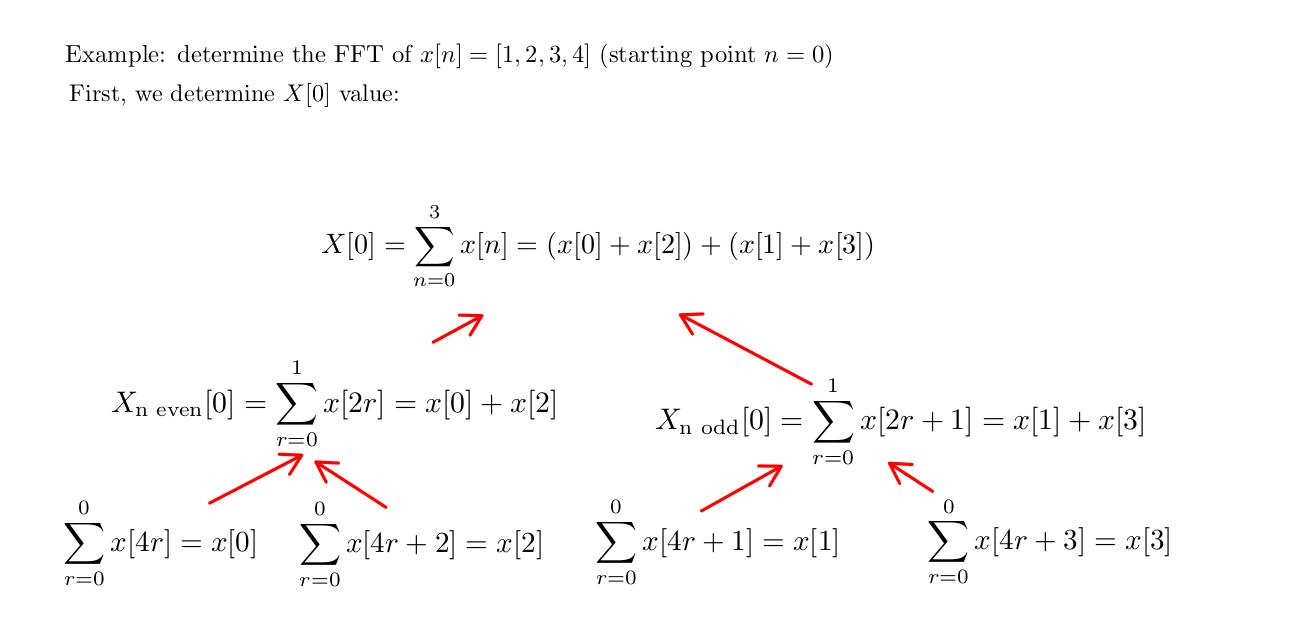
\includegraphics[width=1.1\textwidth]{5.jpg}

			\caption{FFT example}			\label{fig:re5}

		\end{figure}

\end{frame}
\begin{frame}{Biến đổi Fourier nhanh (FFT)}
\begin{figure}[h]
			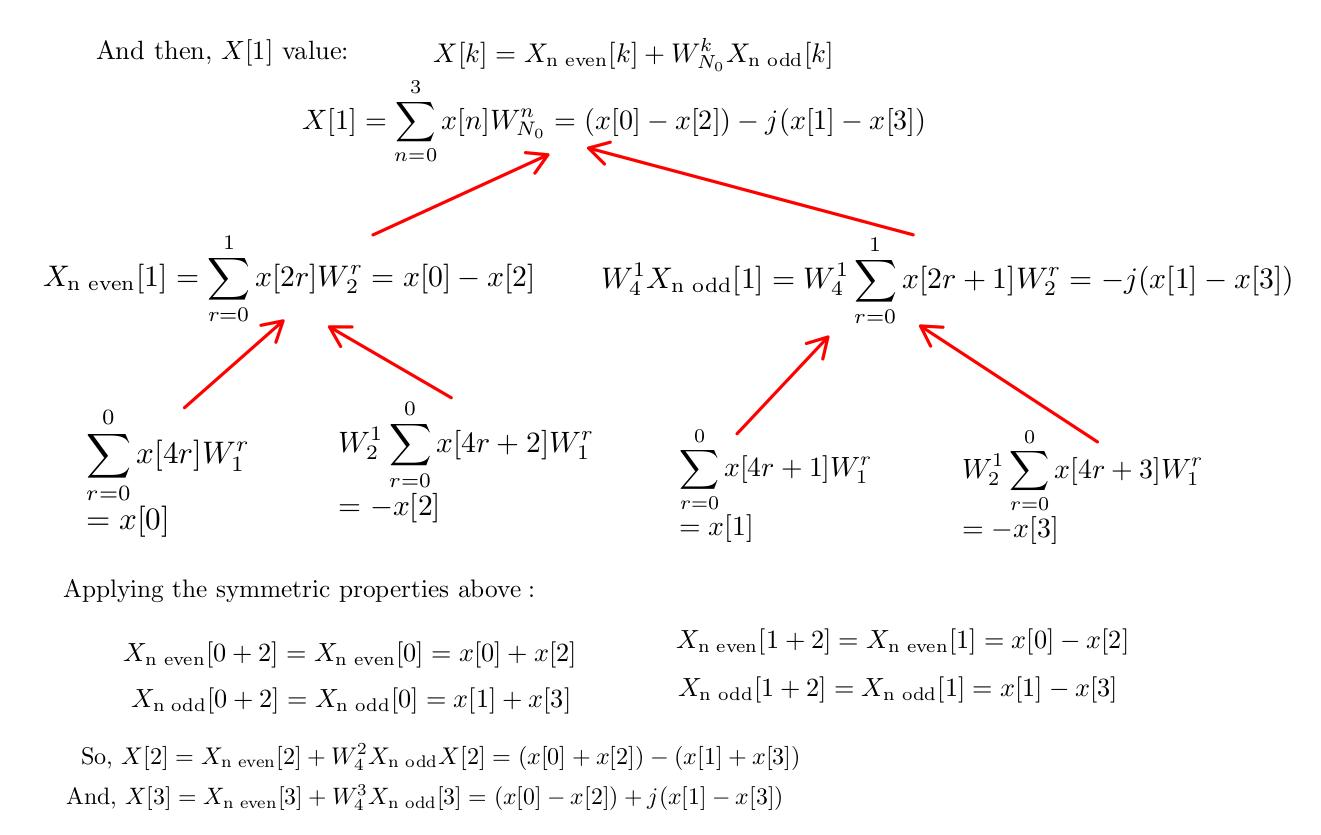
\includegraphics[width=1.1\textwidth]{6.jpg}

			\caption{FFT example}			\label{fig:re6}

		\end{figure}

\end{frame}
\begin{frame}{Biến đổi Fourier nhanh (FFT)}
Từ các kết quả trên, ta tổng hợp lại được:
\begin{equation*}
\begin{split}
	X[0]&=(x[0]+x[2])+(x[1]+x[3])=X_{\text{n even}}[0]+X_{\text{n odd}}[0]\\
	X[1]&=(x[0]-x[2])-j(x[1]-x[3])=X_{\text{n even}}[1]+W_{4}^{1}X_{\text{n odd}}[1]\\
	X[2]&=(x[0]+x[2])-(x[1]+x[3])=X_{\text{n even}}[0]+W_{4}^{2}X_{\text{n odd}}[0]\\
X[3]&=(x[0]-x[2])+j(x[1]-x[3])=X_{\text{n even}}[1]+W_{4}^{3}X_{\text{n odd}}[1]\\
\end{split}
\end{equation*}
Hiển nhiên ta thấy rằng từ kết quả trên, số bước tính toán đã giảm đi đáng kể, thay vì tính theo cách nhân ma trận như trên, ta chỉ cần thực hiện \textbf{6 phép cộng} và \textbf{2 phép nhân} rất đơn giản (chỉ là nhân với đơn vị ảo thuần, thậm chí còn không phải nhóm lại phần ảo và thực như cách nhân ma trận).
\\ Ta vẽ lưu đồ dòng chảy tín hiệu (còn gọi là Butterfly diagram) để tính FFT 4 điểm như sau:
\end{frame}
\begin{frame}{Biến đổi Fourier nhanh (FFT)}
\begin{figure}[h]
			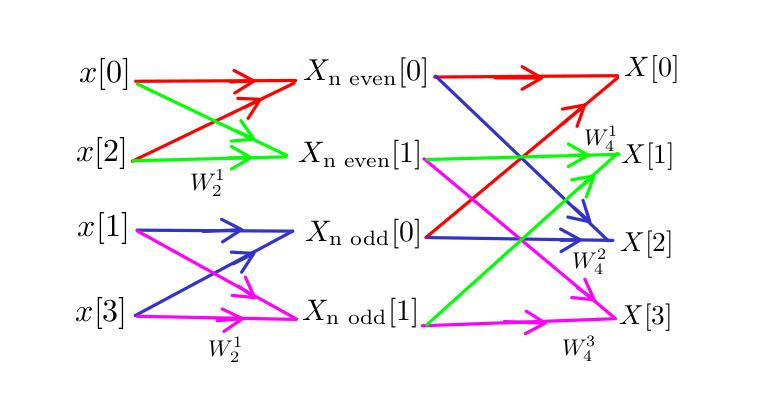
\includegraphics[width=1.1\textwidth]{7.jpg}

			\caption{FFT 4 points Butterfly diagram}			\label{fig:re7}

		\end{figure}
\end{frame}
\begin{frame}{Biến đổi Fourier nhanh (FFT)}
\begin{figure}[h]
			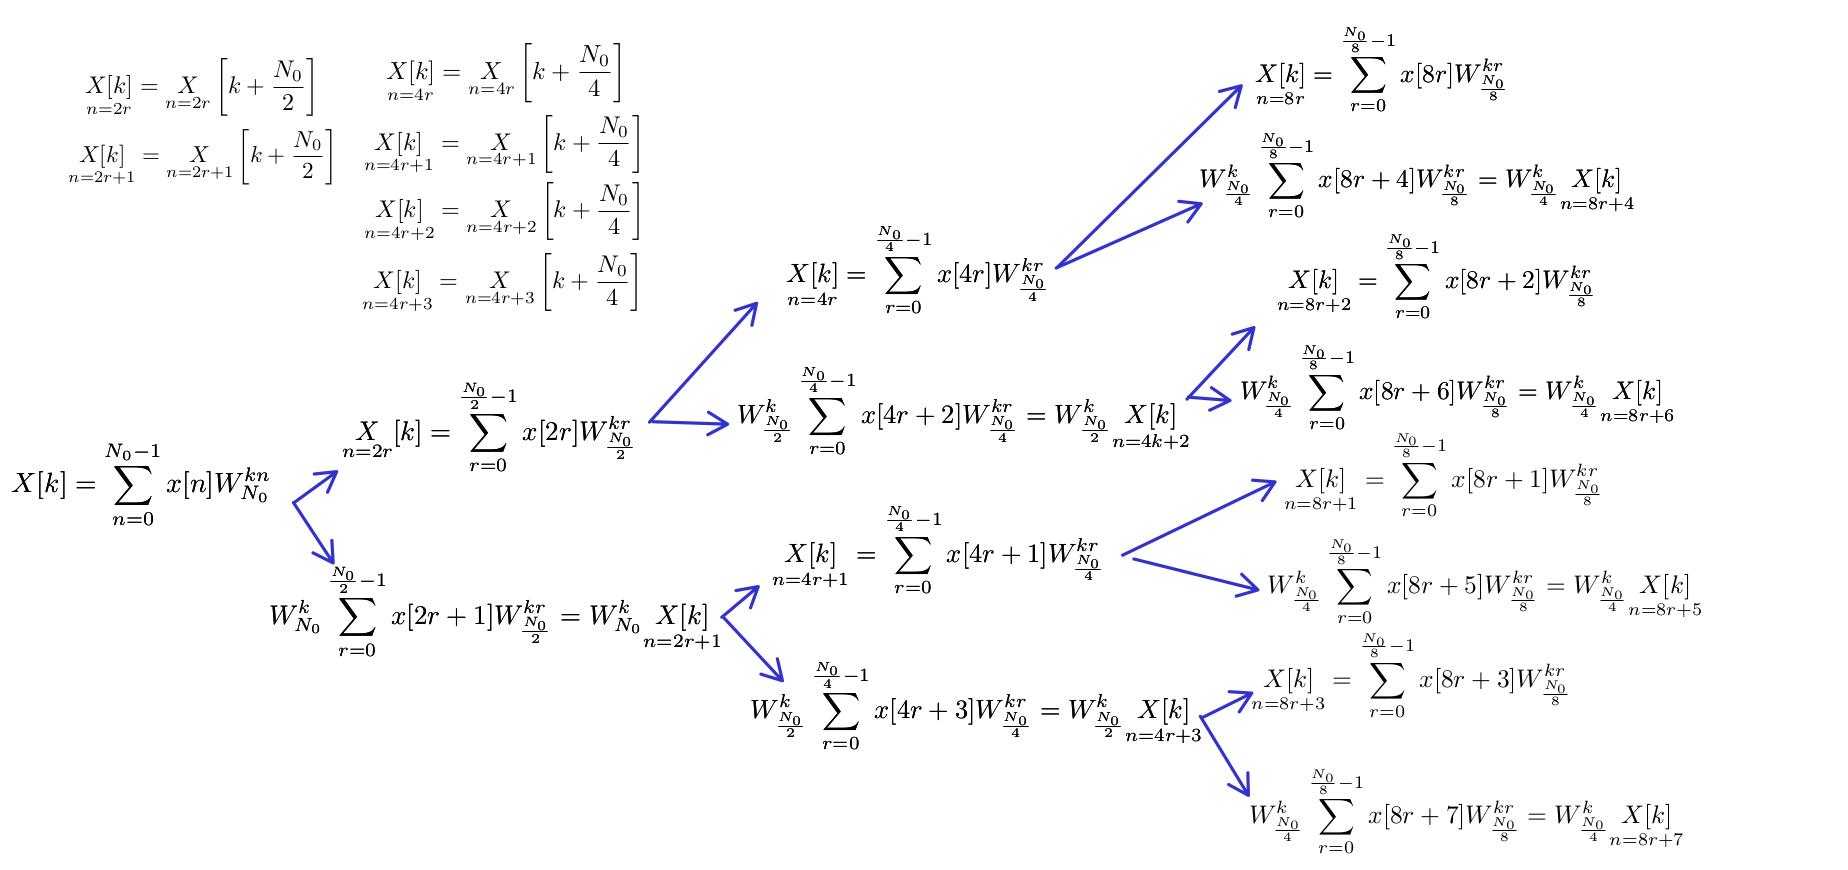
\includegraphics[width=1.1\textwidth]{8.jpg}

			\caption{FFT 8 points}			\label{fig:re8}

		\end{figure}
\end{frame}
\begin{frame}{Biến đổi Fourier nhanh (FFT)}
\begin{figure}[h]
			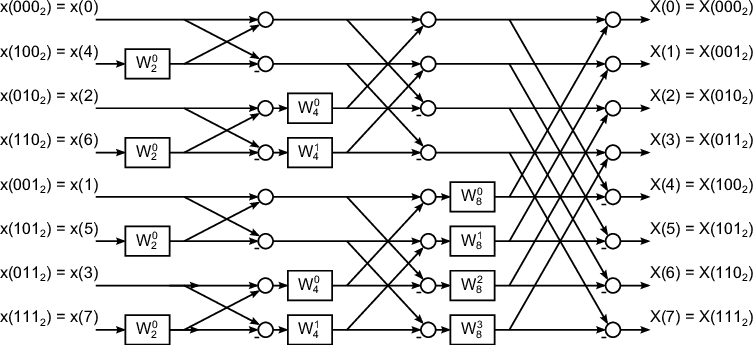
\includegraphics[width=1\textwidth]{9.png}

			\caption{FFT 8 points Butterfly diagram}			\label{fig:re9}

		\end{figure}

\end{frame}
\begin{frame}{Biến đổi Fourier nhanh (FFT)}
Nếu ta thay $W_{N_{0}}^{rk}$ thành liên hợp của nó $W_{N_{0}}^{-rk}=(W_{N_{0}}^{rk})^*$ trong các công thức và lưu đồ tín hiệu, sau đó chia toàn bộ kết quả cho $N_{0}$, ta thu được thuật toán IFFT hoàn toàn tương tự với FFT.
\end{frame}
\end{document}
